\subsection{Teilaufgabe 2}
\subsubsection{Aufgabenstellung}
In dieser Teilaufgabe sollen wir ein Programm schreiben welle die Wertebereiche der primitieven
Datentypen ausgibt.

\subsubsection{Anforderungsdefinition}
\begin{enumerate}
	\item Zu jedem primitieven Datentypen den Max und Min-Wert ausgeben.
\end{enumerate}

\subsubsection{Entwurf}
% generated by Plantuml 1.2018.13      
\definecolor{plantucolor0000}{RGB}{0,0,0}
\definecolor{plantucolor0001}{RGB}{254,254,206}
\definecolor{plantucolor0002}{RGB}{168,0,54}
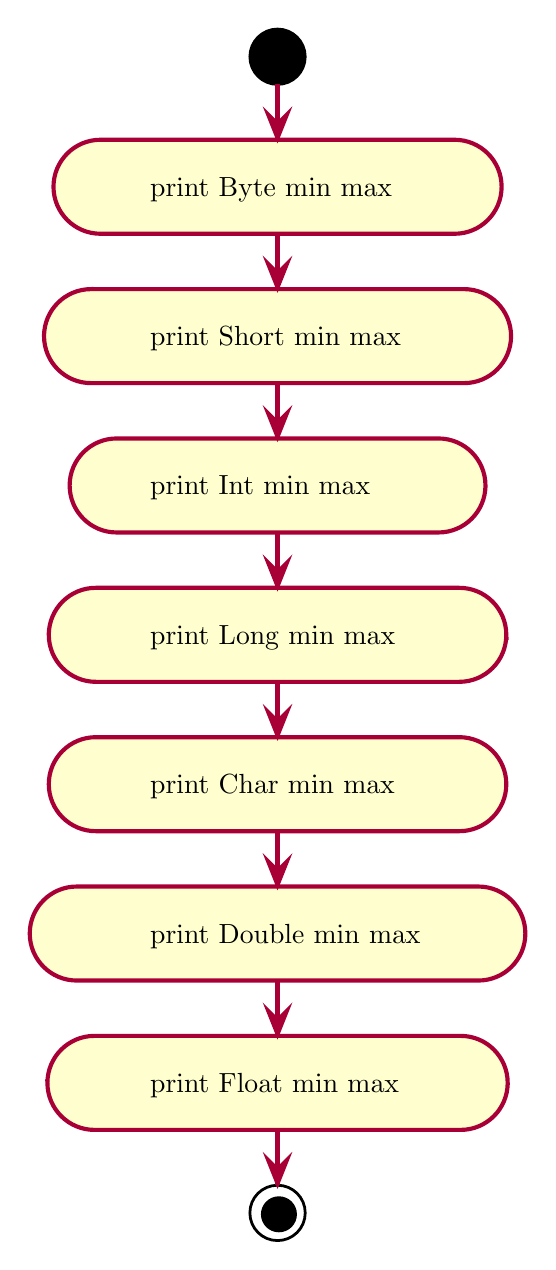
\begin{tikzpicture}[yscale=-1
,pstyle0/.style={fill=black,line width=1.0pt}
,pstyle1/.style={color=plantucolor0002,fill=plantucolor0001,line width=1.5pt}
,pstyle3/.style={color=plantucolor0002,line width=1.5pt}
,pstyle4/.style={color=plantucolor0002,fill=plantucolor0002,line width=1.0pt}
]
\draw[pstyle0] (99.5412pt,20pt) ellipse (10pt and 10pt);
\draw[pstyle1] (18.5775pt,66.9844pt) arc (180:270:16.9844pt) -- (35.5619pt,50pt) -- (163.5204pt,50pt) arc (270:360:16.9844pt) -- (180.5048pt,66.9844pt) -- (180.5048pt,66.9844pt) arc (0:90:16.9844pt) -- (163.5204pt,83.9688pt) -- (35.5619pt,83.9688pt) arc (90:180:16.9844pt) -- (18.5775pt,66.9844pt) -- cycle;
\node at (50pt,60pt)[below right,color=black]{print Byte min max};
\draw[pstyle1] (15.1634pt,120.9531pt) arc (180:270:16.9844pt) -- (32.1478pt,103.9688pt) -- (166.9346pt,103.9688pt) arc (270:360:16.9844pt) -- (183.919pt,120.9531pt) -- (183.919pt,120.9531pt) arc (0:90:16.9844pt) -- (166.9346pt,137.9375pt) -- (32.1478pt,137.9375pt) arc (90:180:16.9844pt) -- (15.1634pt,120.9531pt) -- cycle;
\node at (50pt,113.9688pt)[below right,color=black]{print Short min max};
\draw[pstyle1] (24.4139pt,174.9219pt) arc (180:270:16.9844pt) -- (41.3983pt,157.9375pt) -- (157.6841pt,157.9375pt) arc (270:360:16.9844pt) -- (174.6684pt,174.9219pt) -- (174.6684pt,174.9219pt) arc (0:90:16.9844pt) -- (157.6841pt,191.9063pt) -- (41.3983pt,191.9063pt) arc (90:180:16.9844pt) -- (24.4139pt,174.9219pt) -- cycle;
\node at (50pt,167.9375pt)[below right,color=black]{print Int min max};
\draw[pstyle1] (16.8831pt,228.8906pt) arc (180:270:16.9844pt) -- (33.8675pt,211.9063pt) -- (165.2149pt,211.9063pt) arc (270:360:16.9844pt) -- (182.1992pt,228.8906pt) -- (182.1992pt,228.8906pt) arc (0:90:16.9844pt) -- (165.2149pt,245.875pt) -- (33.8675pt,245.875pt) arc (90:180:16.9844pt) -- (16.8831pt,228.8906pt) -- cycle;
\node at (50pt,221.9063pt)[below right,color=black]{print Long min max};
\draw[pstyle1] (16.8794pt,282.8594pt) arc (180:270:16.9844pt) -- (33.8638pt,265.875pt) -- (165.2186pt,265.875pt) arc (270:360:16.9844pt) -- (182.203pt,282.8594pt) -- (182.203pt,282.8594pt) arc (0:90:16.9844pt) -- (165.2186pt,299.8438pt) -- (33.8638pt,299.8438pt) arc (90:180:16.9844pt) -- (16.8794pt,282.8594pt) -- cycle;
\node at (50pt,275.875pt)[below right,color=black]{print Char min max};
\draw[pstyle1] (10pt,336.8281pt) arc (180:270:16.9844pt) -- (26.9844pt,319.8438pt) -- (172.098pt,319.8438pt) arc (270:360:16.9844pt) -- (189.0824pt,336.8281pt) -- (189.0824pt,336.8281pt) arc (0:90:16.9844pt) -- (172.098pt,353.8125pt) -- (26.9844pt,353.8125pt) arc (90:180:16.9844pt) -- (10pt,336.8281pt) -- cycle;
\node at (50pt,329.8438pt)[below right,color=black]{print Double min max};
\draw[pstyle1] (16.3831pt,390.7969pt) arc (180:270:16.9844pt) -- (33.3675pt,373.8125pt) -- (165.7149pt,373.8125pt) arc (270:360:16.9844pt) -- (182.6992pt,390.7969pt) -- (182.6992pt,390.7969pt) arc (0:90:16.9844pt) -- (165.7149pt,407.7813pt) -- (33.3675pt,407.7813pt) arc (90:180:16.9844pt) -- (16.3831pt,390.7969pt) -- cycle;
\node at (50pt,383.8125pt)[below right,color=black]{print Float min max};
\draw[color=black,line width=1.0pt] (99.5412pt,437.7813pt) ellipse (10pt and 10pt);
\draw[pstyle0] (100.0412pt,438.2813pt) ellipse (6pt and 6pt);
\draw[pstyle3] (99.5412pt,30pt) -- (99.5412pt,50pt);
\draw[pstyle4] (95.5412pt,40pt) -- (99.5412pt,50pt) -- (103.5412pt,40pt) -- (99.5412pt,44pt) -- cycle;
\draw[pstyle3] (99.5412pt,83.9688pt) -- (99.5412pt,103.9688pt);
\draw[pstyle4] (95.5412pt,93.9688pt) -- (99.5412pt,103.9688pt) -- (103.5412pt,93.9688pt) -- (99.5412pt,97.9688pt) -- cycle;
\draw[pstyle3] (99.5412pt,137.9375pt) -- (99.5412pt,157.9375pt);
\draw[pstyle4] (95.5412pt,147.9375pt) -- (99.5412pt,157.9375pt) -- (103.5412pt,147.9375pt) -- (99.5412pt,151.9375pt) -- cycle;
\draw[pstyle3] (99.5412pt,191.9063pt) -- (99.5412pt,211.9063pt);
\draw[pstyle4] (95.5412pt,201.9063pt) -- (99.5412pt,211.9063pt) -- (103.5412pt,201.9063pt) -- (99.5412pt,205.9063pt) -- cycle;
\draw[pstyle3] (99.5412pt,245.875pt) -- (99.5412pt,265.875pt);
\draw[pstyle4] (95.5412pt,255.875pt) -- (99.5412pt,265.875pt) -- (103.5412pt,255.875pt) -- (99.5412pt,259.875pt) -- cycle;
\draw[pstyle3] (99.5412pt,299.8438pt) -- (99.5412pt,319.8438pt);
\draw[pstyle4] (95.5412pt,309.8438pt) -- (99.5412pt,319.8438pt) -- (103.5412pt,309.8438pt) -- (99.5412pt,313.8438pt) -- cycle;
\draw[pstyle3] (99.5412pt,353.8125pt) -- (99.5412pt,373.8125pt);
\draw[pstyle4] (95.5412pt,363.8125pt) -- (99.5412pt,373.8125pt) -- (103.5412pt,363.8125pt) -- (99.5412pt,367.8125pt) -- cycle;
\draw[pstyle3] (99.5412pt,407.7813pt) -- (99.5412pt,427.7813pt);
\draw[pstyle4] (95.5412pt,417.7813pt) -- (99.5412pt,427.7813pt) -- (103.5412pt,417.7813pt) -- (99.5412pt,421.7813pt) -- cycle;
\end{tikzpicture}


\subsubsection{Quelltext}
\paragraph{Wertebereiche.java}\
\lstinputlisting[language = Java , frame = trBL , escapeinside={(*@}{@*)}]{../chapter_03/src/chapter_03/Wertebereiche.java}


\subsubsection{Testdokumentation}


\subsubsection{Benutzungshinweise}
Keine Besonderen Benutzungshinweise.
Man navigiere zu dem Ordner von sich die Compilierte Datei mit dem Namen "Wertebereiche.class"
\space befindet und führt anschlie\ss end java Wertebereiche aus.

\subsubsection{Anwendungsbeispiel}
Nach dem man das Programm gestartet hat, sollte folgende Ausgabe erscheinen:
\begin{lstlisting}[frame = trBL , firstnumber = last , escapeinside={(*@}{@*)}]
[sebastian@laptop bin]$ java Wertebereiche
Byte min -128 | Byte max 127
Short min -32768 | Short max 32767
Integer min -2147483648 | Integer max 2147483647
Long min -9223372036854775808 | Byte Long 9223372036854775807
Char min  | Char max ￿
Float min 1.4E-45 | Float max 3.4028235E38
Double min 4.9E-324 | Double max 1.7976931348623157E308
[sebastian@laptop bin]$ 
\end{lstlisting}